\chapter{Information and Communication Technologies for Developing Countries}
\section{In General}
No correlation with productivity \cite{rh:isdc}

\begin{quotation}
Lack of literature in general: Until very recently,
the entire literature on IS and developing countries
would struggle to ll a single bookshelf. The
attention of writers—from researchers to consultants
to journalists—has been focused elsewhere.\cite{rh:isdc}
\end{quotation}
\begin{quotation}
Lack of evaluation: Those who have the will to
evaluate—such as academics—often lack the
resources and capacity. Those who have the
resources—such as aid donor agencies—often
lack the will to evaluate.\cite{rh:isdc}
\end{quotation}
\begin{quotation}
Focus on case studies: The literature on IS in
DCs has grown, but it is a literature dominated by
case studies of individua l IS projects. Taken alone,
these provide no basis for estimation of overall
failure/success rates.\cite{rh:isdc}
\end{quotation}


\section{Updated Information}

\section{The design and actuality gap}

\begin{figure}
\centering
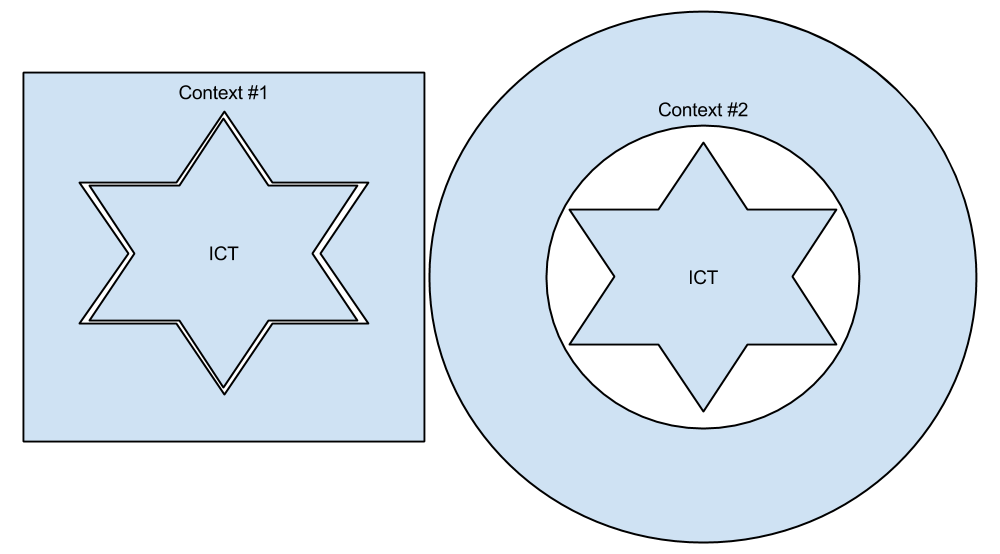
\includegraphics[width=\columnwidth]{literature/ict_in_dev/images/contextIctProblem.png}
\label{cip}
\caption{If it works for us it will work for you!}
\end{figure}

\section{Success or Failure}

\begin{figure}
\centering
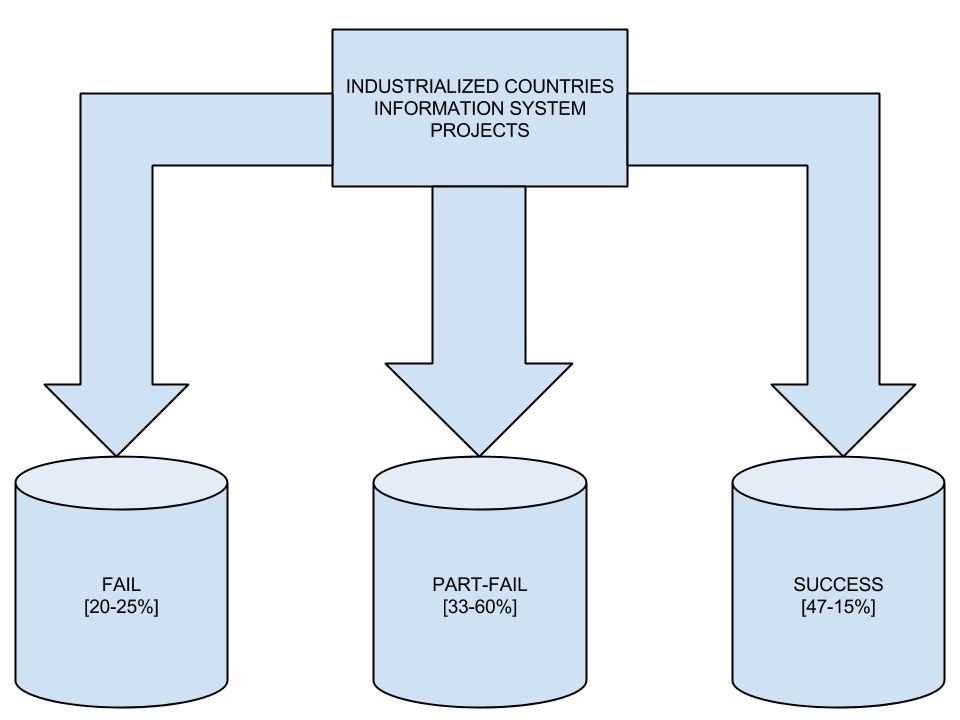
\includegraphics[width=\columnwidth]{literature/ict_in_dev/images/iCountryISProjects(1995-2000).png}
\label{icisp}
\caption{IS projects in Industrialized Countries. Year: 1995-2000 \cite{rh:isdc}}
\end{figure}

Find the common thread in both.

\section{Success stories}
\subsection{short examples}
\section{Failure stories}
\subsection{short examples}

\section{Evidence base}

\begin{quotation}
Health information systems in South Africa: Braa
and Hedberg (2002) reported widespread partial
failure of high cost systems with little use of data.\cite{rh:isdc}
\end{quotation}

\begin{quotation}
IS in the Thai public sector: Kitiyadisai (2000)
reported “failure cases seem to be the norm in
Thailand at all governmental levels.”\cite{rh:isdc}
\end{quotation}

\begin{quotation}
Donor-funded IT projects in China: Baark and
Heeks (1999) reported that all were found to be
partial failures.\cite{rh:isdc}
\end{quotation}

\begin{quotation}
World Bank-funded IT projects in Africa: Moussa
and Schware (1992) reported almost all as partial—
often sustainability—failures.\cite{rh:isdc}
\end{quotation}


\section{Digital Divide}

\section{The illusion of a computer being something else than a calculator}

\section{Implicit and explicit components of Design}
The explicit components of a computer application is the physical components the user would need in order to use the application.
Examples include cost, computer hardware, operating system, monitor and such.
The implicit ones are a little harder to quantify. These include knowledge, expectations and skill.
When addressing the implicit, how would one go about evaluating if the user is qualified to use the application as intended and ensure that it is used for the proper intentions?  

